\entry{Semana del 25/08/2025.} 

\section{Lunes 25/08/2025.}  

\subsection*{Notas del día:}  
\begin{itemize}
	\setlength\itemsep{0.1em}
	\item Voy a medir hoy con FCD. 
	\item Armé todo en la cuba grande, tuve que mover la LED con el patrón a uno de los bordes porque en el centro no le daba el largo al vástago del motor. 
	\item Para la cámara la lente que usamos es la de 18/105, a la de 55 no le daba el zoom/enfoque a la altura que queríamos. 
	\item Juan y Mateo armaron para que el aptrón quede pegado al borde de la cuba, así que no hay distancia de aire en el medio. 
	
	\item Nos quedan entonces: Piso cuba grande (1.2 cm), piso cuba chica (1 cm), altura de agua en equilibrio (5.7 cm). 
	\item Paleta sumergida unos 1.8 cm. 
	
	\item Shutter 1/2000 y 250 fps. 
	\item Patrón 2 mm por cuadradito. 
	\item La paleta en el forzado va giirando un poco. 
	
	\item Voy a medir para el forzado entre 0 y 4 Hz y amplitudes: 50 \% (referencia 1), 20 \% (referenica 2), 60 \% (referencia 2), 40 \%, 30 \% (referencia 3), 10 \% (referencia 3), 70 \%. 
	\item Referencia 2 justo entre las dos mediciones. 
	
\end{itemize}

\subsection*{Reconstrucción de la superficie libre con FCD en forzado aleatorio.}

Ahora en lugar de utilizar el sensor capacitivo repetí algunas de las experiencias del Viernes pasado pero midiendo la superficie libre con FCD. Acá forcé siempre entre 0 y 4 Hz y solo varié la amplitud entre 10 \% y 70 \%. El Setup es el que está descripto más abajo. 

\begin{figure}[!ht]
	\begin{minipage}[c]{0.5\textwidth}
			\begin{subfigure}{\textwidth}
					\centering
					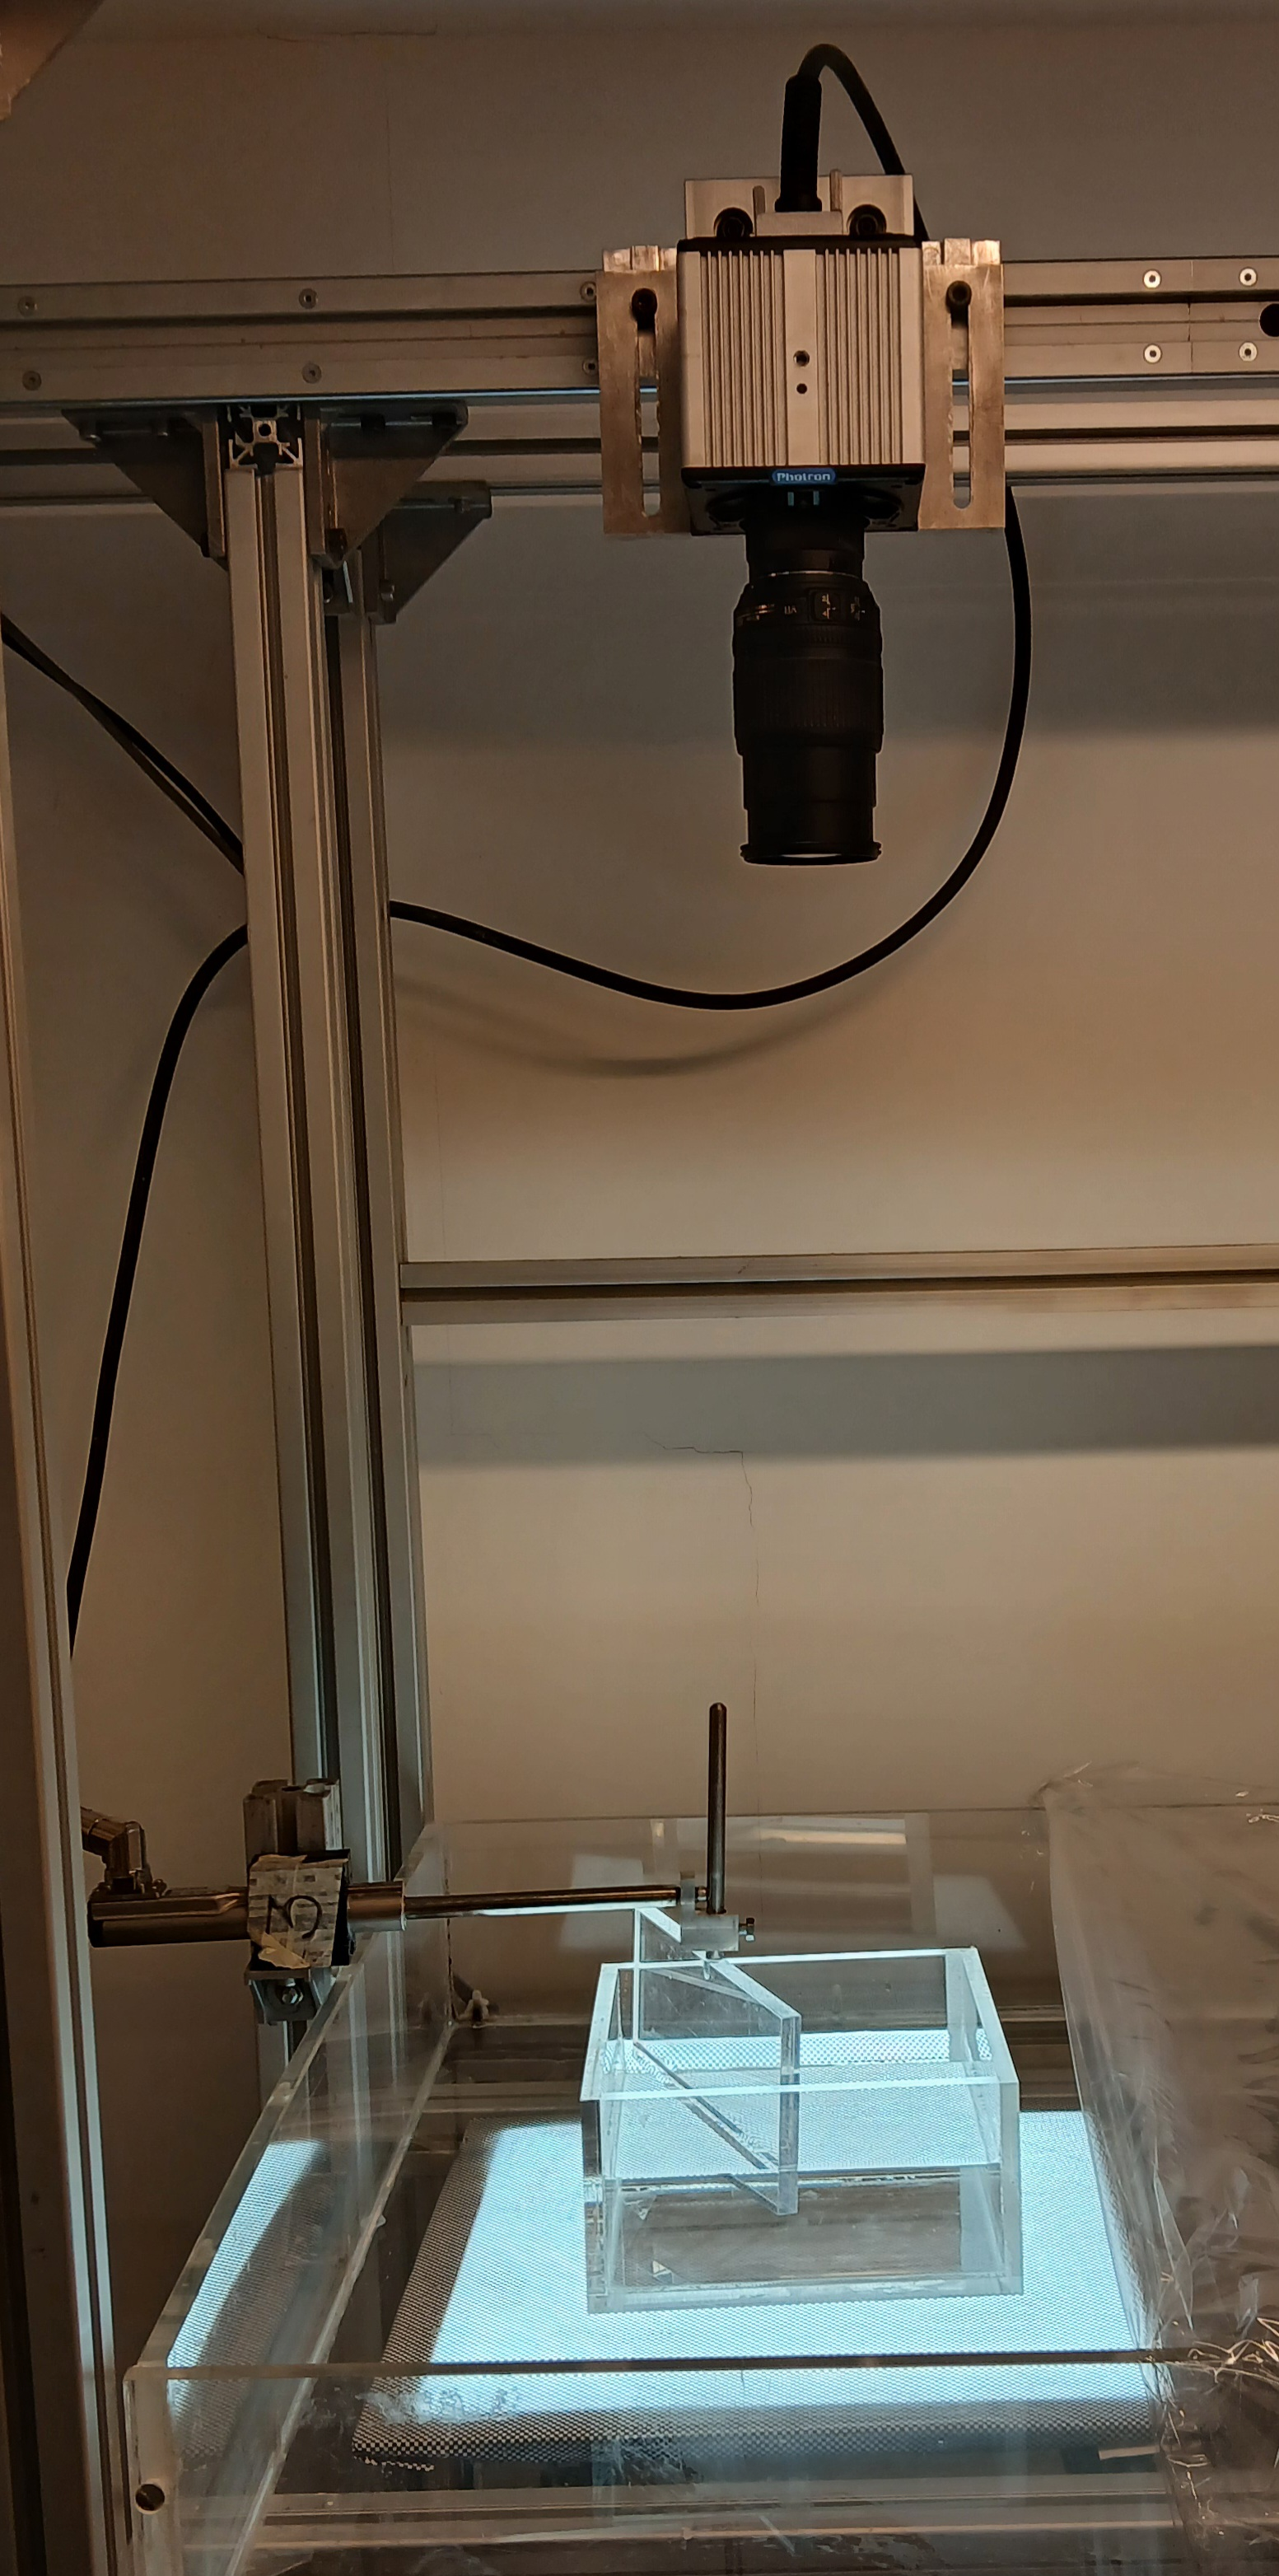
\includegraphics[width=0.341568\textwidth]{Figures/25_08_2025/Setup_cuba_chica_FCD.jpg}
					\captionsetup{width=0.8\textwidth}
					\subcaption{Vista lateral.}
				\end{subfigure}
		\end{minipage}\begin{minipage}[c]{0.49\textwidth}
			\begin{subfigure}{\textwidth}
					\centering
					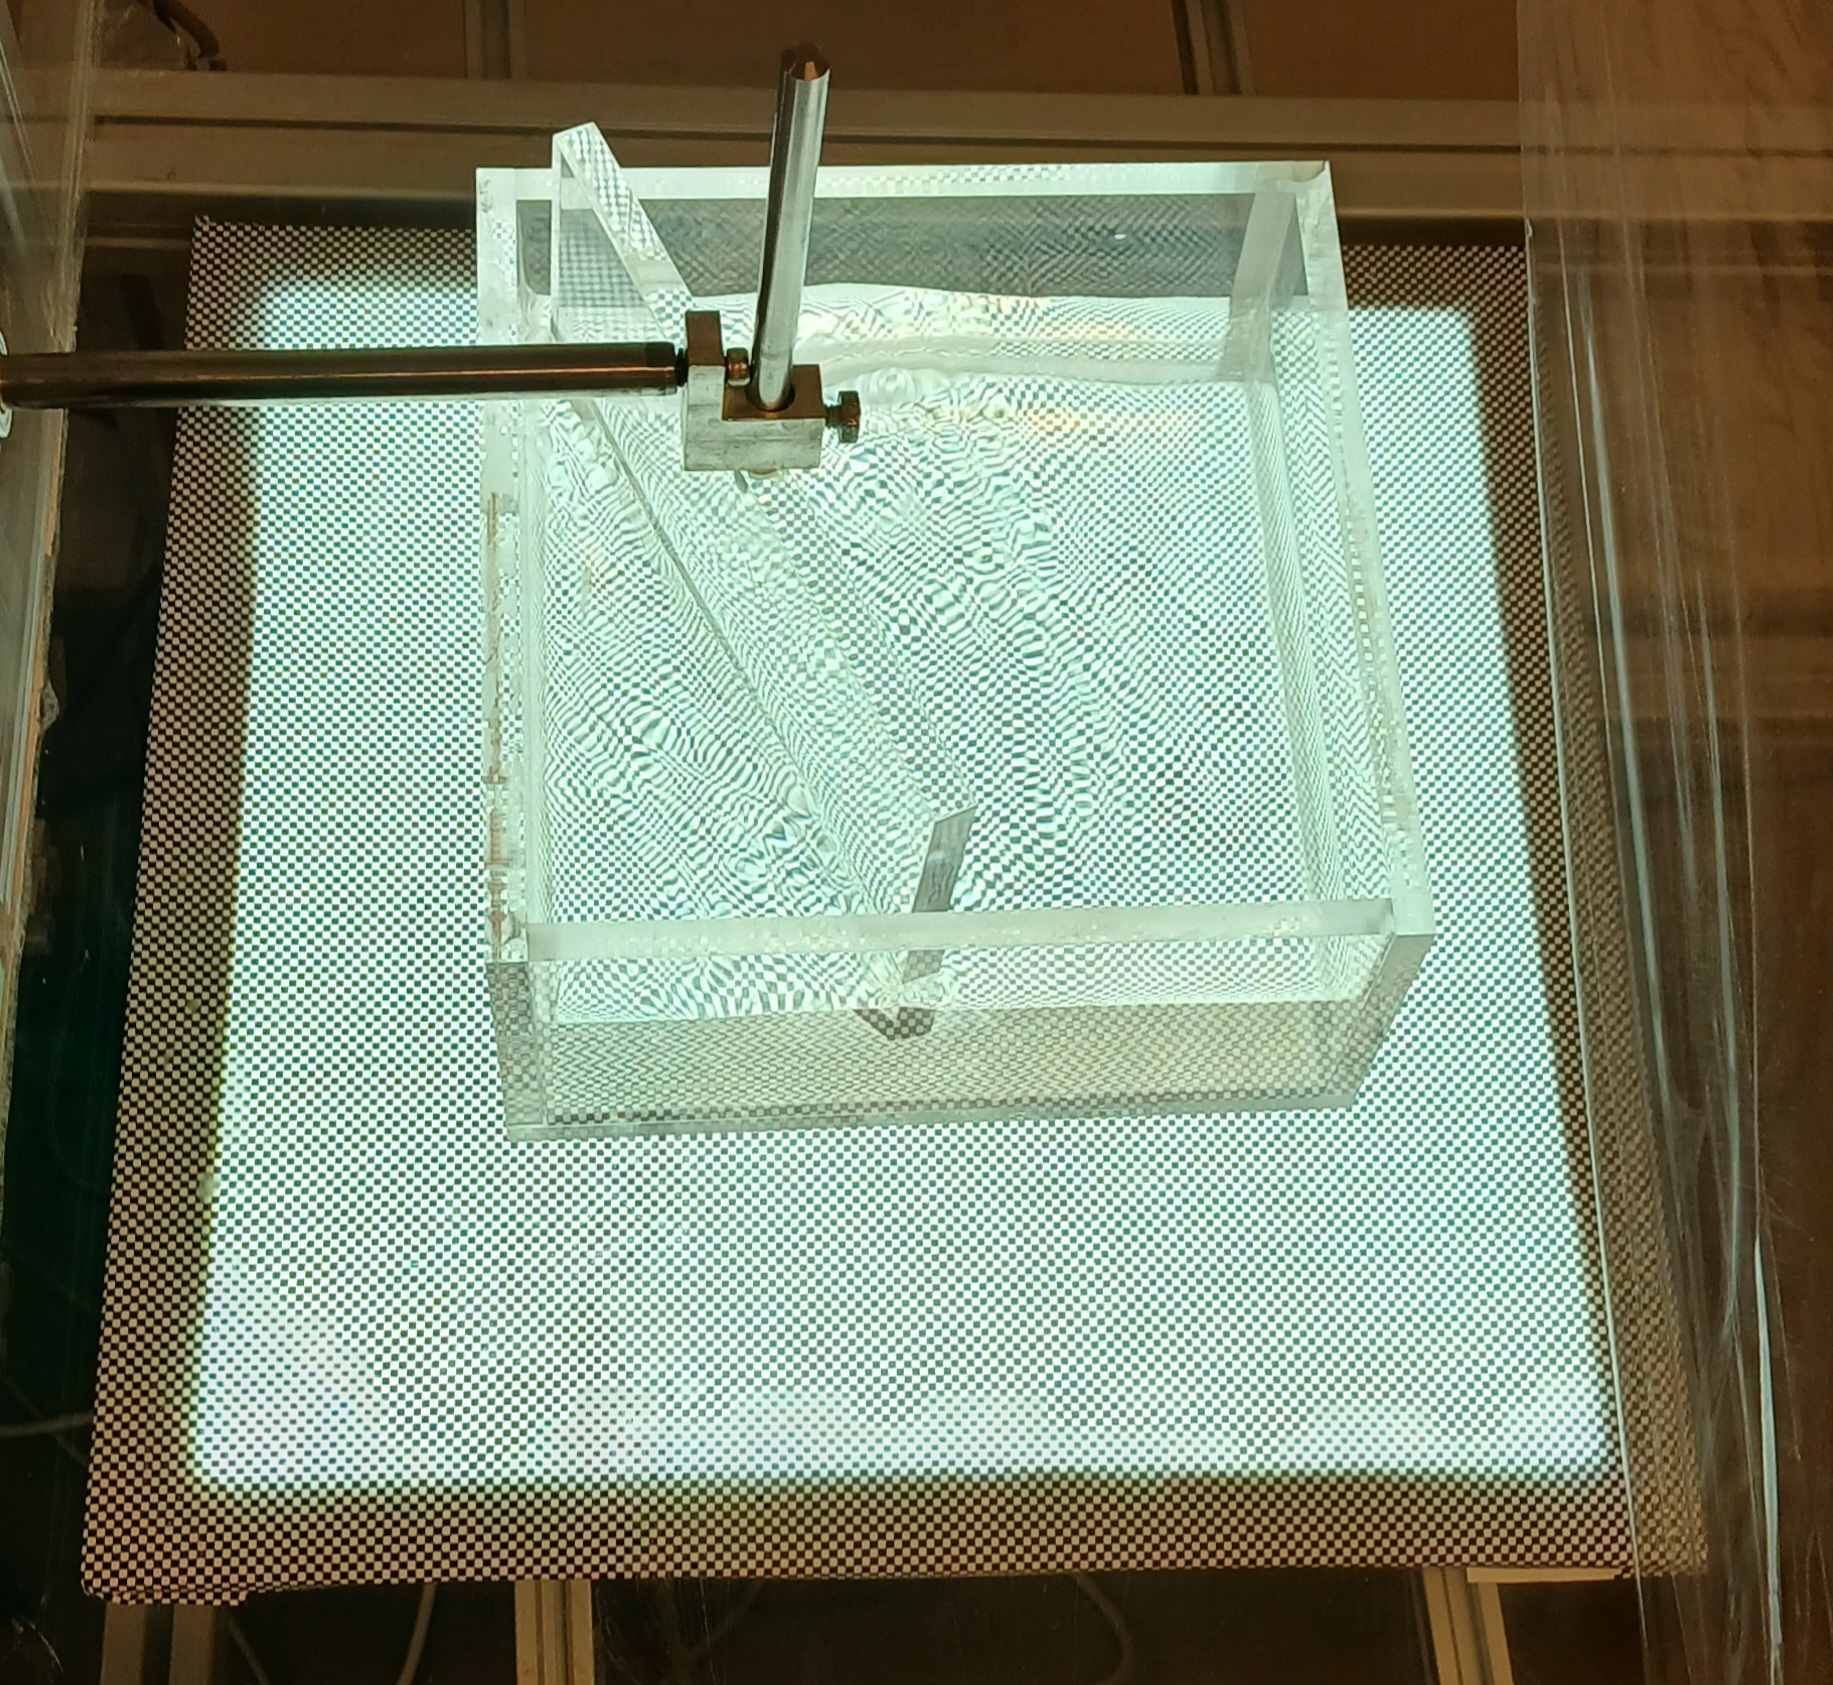
\includegraphics[width=0.678\textwidth]{Figures/25_08_2025/Setup_cuba_chica_FCD_detalle.jpg}
					\captionsetup{width=0.8\textwidth}
					\subcaption{Vista superior.}
				\end{subfigure}
		\end{minipage}
	\caption{Setup para estudiar la respuesta del fluido en la cuba chica a un forzado aleatorio entre 0 y 4 Hz para varias amplitudes utilizando un único wave-driver. Acá mido una sección de la superficie libre, reconstruyendo la topología completamente mediante FCD, utilizando la cámara de alta velocidad (a 250 fps) para registrar la deformación del patrón cuadriculado que se encuentra iluminado por la luz LED debajo del fluido.}
	\label{fig:setup_cuba_chica_FCD}
\end{figure} 

Para la reconstrucción usé el código que habíamos armado el año pasado. Las secciones analizadas fueron de unos 600 x 600 px (siempre cuadradas) y los 3072 frames. Cada video llevó más o menos 1 hora y media en anaizarse. 

A continuación algunos snapshots de los campos de alturas reconstruídos para varias de las amplitudes estudiadas.

\begin{figure}[!ht]
	\begin{minipage}[c]{0.3325\textwidth}
			\begin{subfigure}{\textwidth}
					\centering
					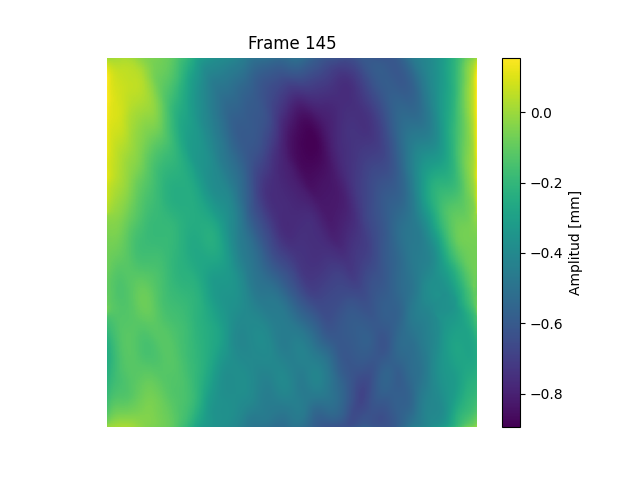
\includegraphics[width=0.98\textwidth]{Figures/25_08_2025/Alturas_amplitud_10.png}
					\captionsetup{width=0.8\textwidth}
					\subcaption{Amplitud 10 \%.}
				\end{subfigure}
		\end{minipage}\begin{minipage}[c]{0.33249\textwidth}
			\begin{subfigure}{\textwidth}
					\centering
					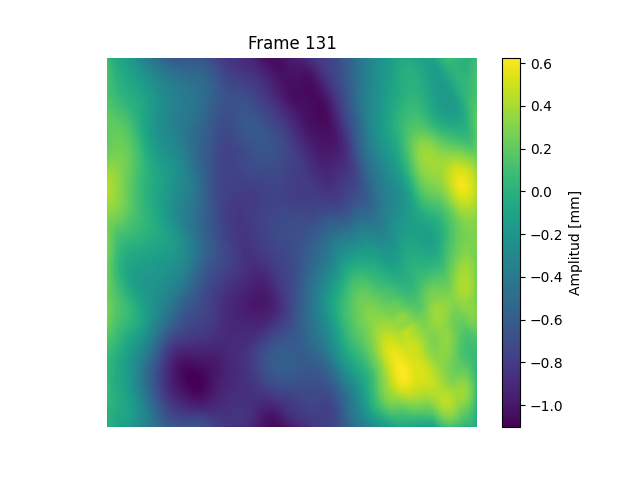
\includegraphics[width=0.98\textwidth]{Figures/25_08_2025/Alturas_amplitud_30.png}
					\captionsetup{width=0.8\textwidth}
					\subcaption{Amplitud 30 \%.}
				\end{subfigure}
		\end{minipage}\begin{minipage}[c]{0.33249\textwidth}
			\begin{subfigure}{\textwidth}
					\centering
					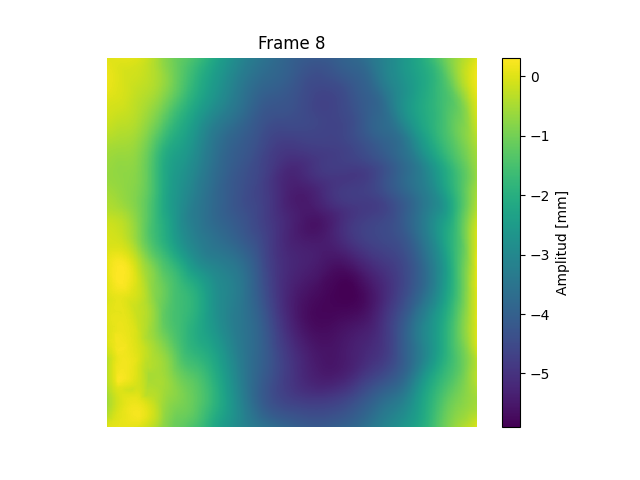
\includegraphics[width=0.98\textwidth]{Figures/25_08_2025/Alturas_amplitud_50.png}
					\captionsetup{width=0.8\textwidth}
					\subcaption{Amplitud 50 \%.}
			\end{subfigure}
		\end{minipage}
	\caption{Algunos ejemplos de la reconstrucción completa de la topografía del campo de alturas por FCD para las distintas amplitudes.}
	\label{fig:ejemplos_Aturas}
\end{figure} 

Durante varios frames parece funcionar correctamente pero después hace cosas raras, y aparecen picos y otros artificios en los resultados, especialmente para las amplitudes más altas. Puede ser que ya esto sea demasiado no lineal para el método que está pensado para el caso lineal, pero aparecen incluso para la amplitud más baja de $10$ \%. 

\section{Miércoles 27/08/2025.} 

\subsection*{Notas del día:} 
\begin{itemize}
	\setlength\itemsep{0.5421em}
	\item Tomé un par de imágenes para ver cómo cambia la calibración según si usamos las medidas de abajo o las de arriba. Y además confirmar si va el factor $\sqrt{2}$ midiendo con la regla a la altura del patrón. 
	\item  Todo en zoom un poco más de 70, reenfocando en cada momento. 
	\item  Altura de cámara (unión con carcasa y lente) hasta base de la cuba es de 89/90 cm medido con metro.  
	
	\item  De FCD da calibration\_factor = 0.00019148936170212765 m/px y de la regla da 11.414965986394558 px/0.5 mm. 
	\item O sea, c\_fcd = 0.19 mm/px y c\_regla = 0.04 mm/px. Hay algo raro con el de la regla. Contando a mano son 5 px/mm, o sea que c\_fcd parece estar bien.
	\item  Con la regla elevada son 6 px/mm ahora, o sea que el factor de calibración se hace más chico. 
	
	\item  El factor de calibración hay que corregirlo como * np.sqrt(2) / 2, ya que la periodicidad es diagonal, un periodo es un cuadrada en diagonal, y el 2 para sacar que de antemano multiplicábamos por 2 por ser 2 cuadrados la longitud de onda, cuando pensaba que era horizontal la periodicidad. 
	\item Resulta finalmente que todo el problema era que en vez de guardar los complejos al hacer la transformada espacial 2D guardaba solo la amplitud. Al guardar los complejos y pasar de usar Welch para la FFT temporal a una normal da bien el escaleo e isotropía con la calibración usual que veníamos usando (que coincide con la que obtengo contando a mano los píxeles en la imagen). 
\end{itemize}

\subsection*{Transformada 3D de $\eta(x, y, t)$.}
Una vez procesados los videos con FCD quedé con los campos $\eta(x, y, t)$. Para procesarlos completamente al no poder cargar todo en memoria lo fui haciendo por aprtes. 

En primer lugar analicé cada frame, haciendo la FFT espacial 2D y guardando las amplitudes complejas $\eta(k_x, k_y, t)$. 

Luego analicé cada pixel, haciendo la FFT temporal 1D, quedando ahora sí con $\eta(k_x, k_y, \omega)$. 

Podemos notar que para cada frecuencia la energía se distribuye de forma bastante isótropa en el espacio $\vec k$, aunque está la dirección privilegiada de la paleta y las reflexiones. Además está especialmente concentrada en el $|\vec k|$ que se corresponde con esa frecuencia mediante la relación de dispersión teórica para las ondas gravito-capilares: 

\begin{equation}
	\omega^2(k) = \left( gk + \frac{\gamma}{\rho}k^3\right)\tanh(kh)
\end{equation}

Abajo algunos ejemplos de esto para la amplitud más baja analizada (del 10 \%). 

\vspace{2.5em} 
\begin{figure}[!ht]
	\begin{minipage}[c]{0.5\textwidth}
			\begin{subfigure}{\textwidth}
					\centering
					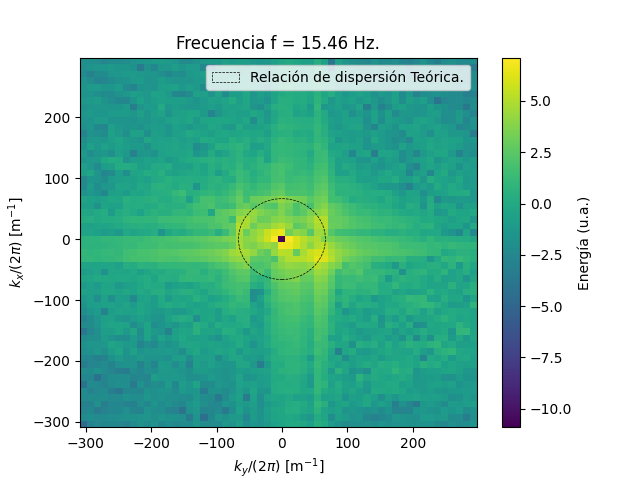
\includegraphics[width=0.98\textwidth]{Figures/25_08_2025/Ejemplo_isotropía_2_amp10.png}
					\captionsetup{width=0.8\textwidth}
				\end{subfigure}
		\end{minipage}\begin{minipage}[c]{0.49\textwidth}
			\begin{subfigure}{\textwidth}
					\centering
					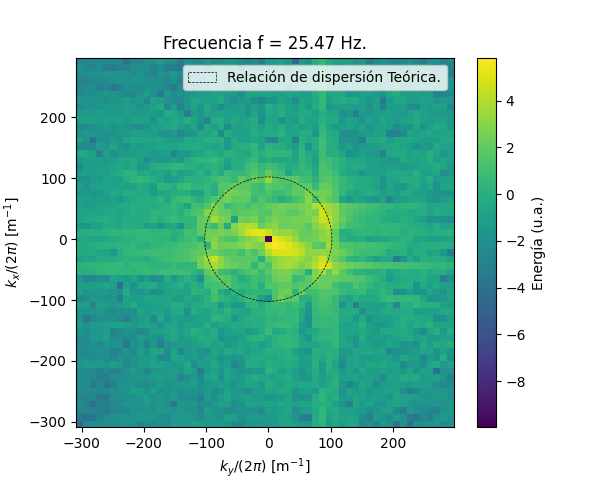
\includegraphics[width=0.98\textwidth]{Figures/25_08_2025/Ejemplo_isotropía_amp10.png}
					\captionsetup{width=0.8\textwidth}
				\end{subfigure}
		\end{minipage}
	\caption{Ejemplos de isotropía en el forzado aleatorio de la cuba chica para amplitud del 10 \%. }
	\label{fig:isotropía_amp10}
\end{figure} 

\vspace{2.5em} 

\subsection*{Espectro promediado y relación de dispersión.} 
Después lo que hice fue hacer un promedio radial para cada frecuencia y armar el mapa completo de $\eta(k,\omega)$ que es lo que está más abajo.

Podemos notar que la región donde se concentra la energía coincide efectivamente con la relación de dispersión como era de esperarse y además pareciera ser que se va difuminando la misma, lo que nos indicaría que la región donde se encuentra se va ensanchando a causa de los efectos no lineales que se vuelven más relevantes cuanto más fuerte es el forzado. 

En este caso no se nota que aparezcan ramas de la relación de dispersión por \textit{Bound Waves}, como encuentran en \cite{herbertObservationNonlinearDispersion2010}, aunque tenemos baja resolución en $\vec k$ ya que analizamos un área relativamente pequeña. La formas de las ramas para futuras referencias son: 

\begin{equation}
	\Omega_N(k) = N \omega(k/N) 
	\label{eq:ramas_relación_de_disersión} 
\end{equation}

Una nota importante es que cuando al hacer la transformada 2D y guardaba solo la amplitud los resultados era muy parecidos cualitativamente a los de ahora, pero quedaba dando vueltas un factor de escala que hacía que no coincida con la relación de dispersión, y a parte aparecía por encima de la curva más marcada una curva secundaria muy tenue.  


\begin{figure}[!ht] %  
	\centering
	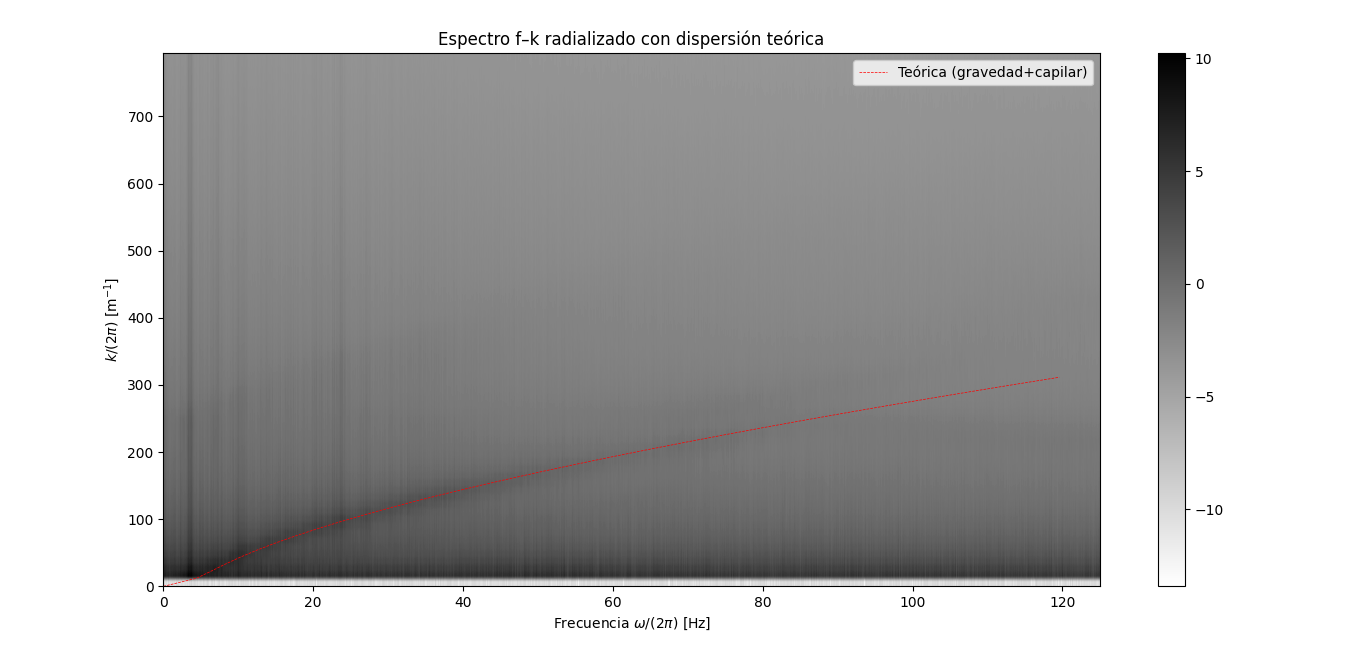
\includegraphics[width=0.897\linewidth]{Figures/25_08_2025/Relación_10}
	
	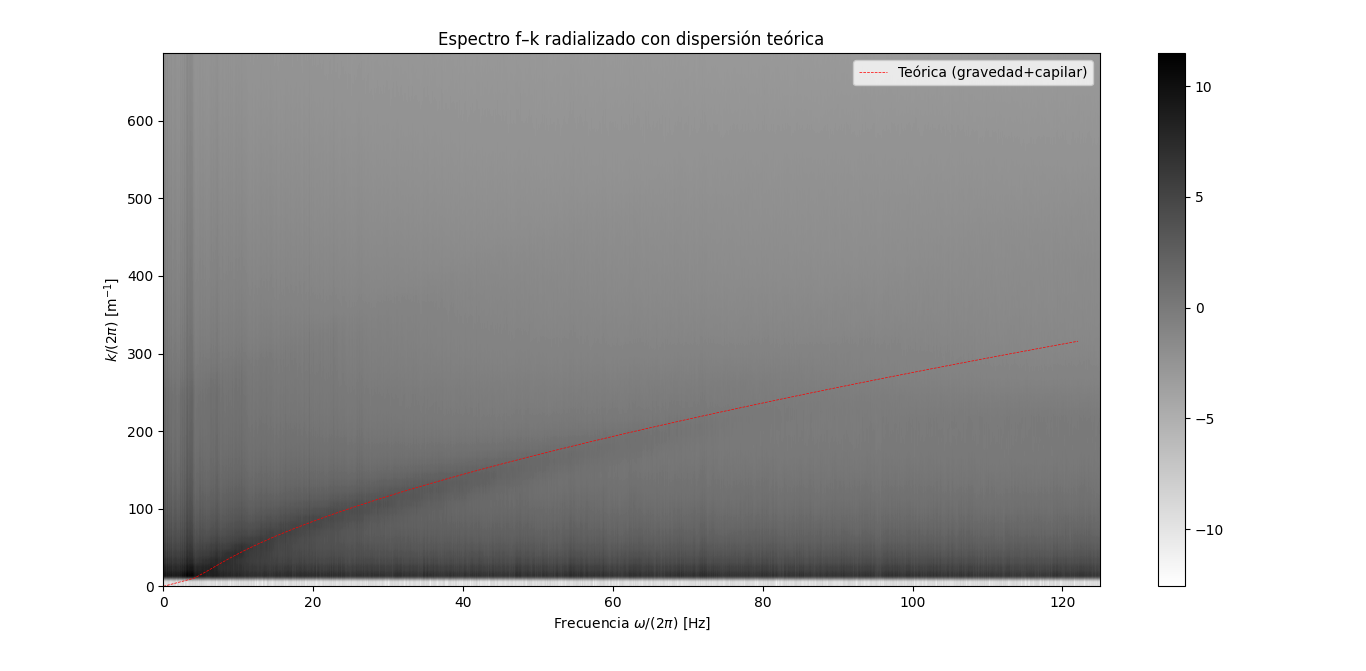
\includegraphics[width=0.897\linewidth]{Figures/25_08_2025/Relación_30}

	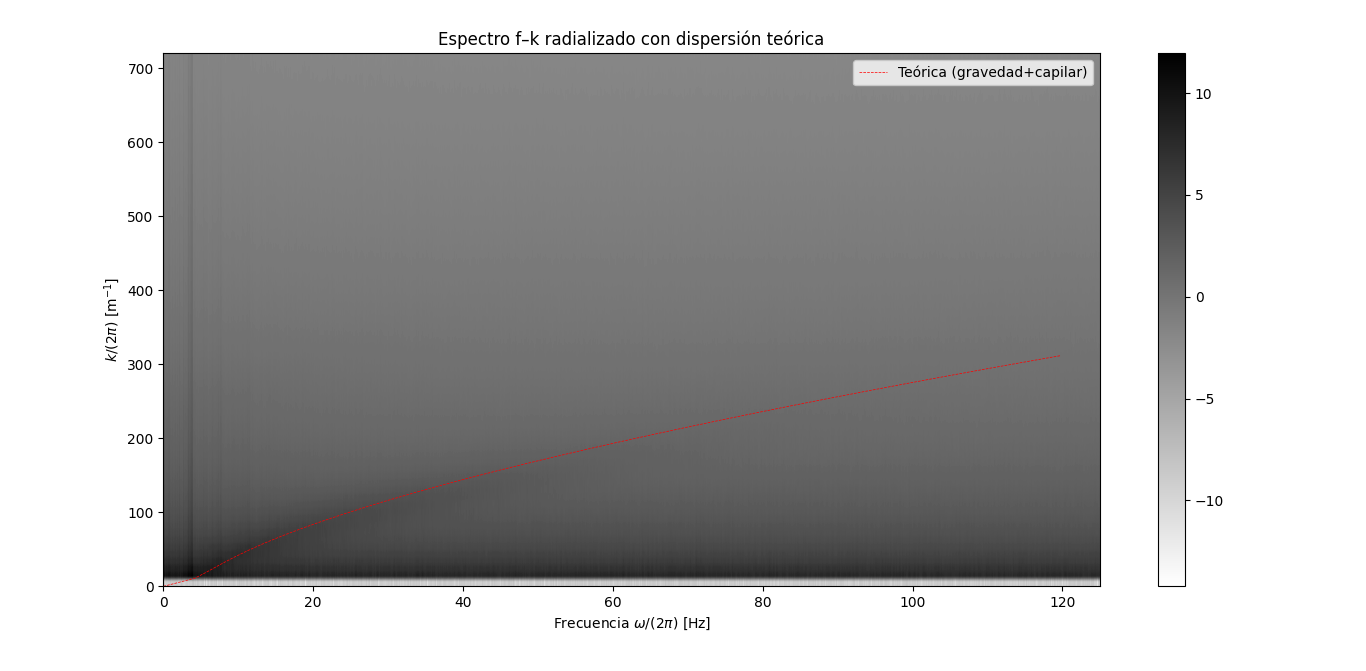
\includegraphics[width=0.897\linewidth]{Figures/25_08_2025/Relación_50}
	
	\caption{Espectro bidimensional $\eta(\omega, |\vec k|)$ para amplitud de forzado  entre 0 y 4 Hz para amplitudes (de arriba a abajo) del 10, 30 y 50 \%.} 
	\label{fig:relacion10}
\end{figure}


\vspace{5.2em} 
\vspace{5.2em} 

\section{Resultados para las mediciones con el sensor capacitivo.} 
Acá seguí bastante lo que está detallado en \cite{falconObservationGravityCapillaryWave2007} para analziar las series temporales. 

\subsection*{PDFs}
Acá están las PDFs para las distintas series temporales, calculadas en ventanas y después promediadas. Se nota que son ligeramente no Gaussianas, y esperaríamos que menos lo sean cuanto más potenciada inyectada en el forzado, ya que aparecen más efectos no lineales. 

En todos los casos están normalizadas por la desviación estándar y tienen media 0.  

\begin{figure}[!ht]
	\begin{minipage}[c]{0.5\textwidth}
			\begin{subfigure}{\textwidth}
					\centering
					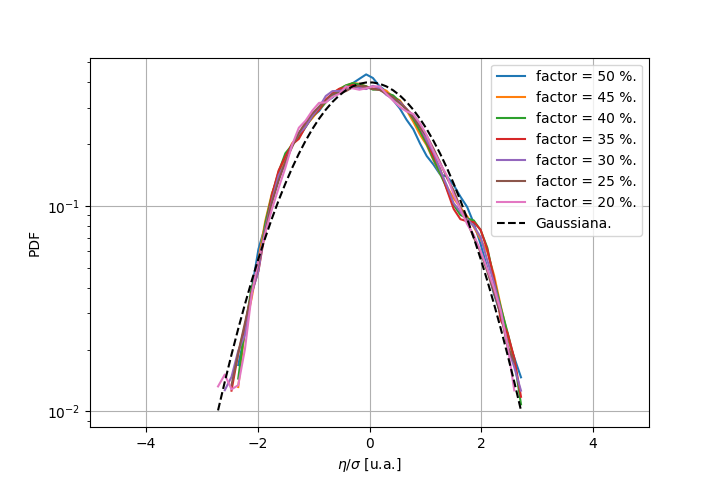
\includegraphics[width=0.98\textwidth]{Figures/25_08_2025/PDFS_variando_amplitud.png}
					\captionsetup{width=0.8\textwidth}
					\subcaption{Amplitud.}
				\end{subfigure}
		\end{minipage}\begin{minipage}[c]{0.49\textwidth}
			\begin{subfigure}{\textwidth}
					\centering
					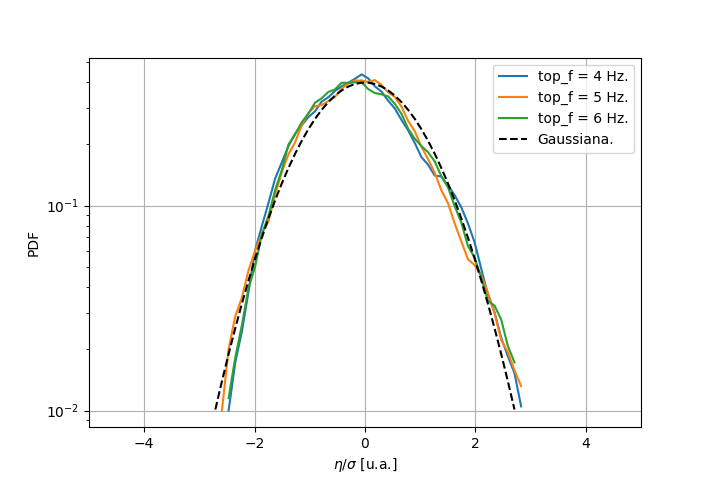
\includegraphics[width=0.98\textwidth]{Figures/25_08_2025/PDFS_variando_frecuencia.png}
					\captionsetup{width=0.8\textwidth}
					\subcaption{Banda de frecuencia.}
				\end{subfigure}
		\end{minipage}
	\caption{PDFS normalizadas por desviación estándar y media 0 para el forzado en la cuba chica en distintas amplitudes (frecuencia de 0 a 4 Hz constante) y para varias bandas de frecuencia (amplitud 50 \% constante).}
	\label{fig:PDFS_sensor}
\end{figure} 

\subsection*{Espectros.}
Acá están los espectros obtenidos por Welch para todas las series temporales. 

Podemos notar que cuanto más potencia inyectamos a más escalas llega la cascada de energía.  

\begin{figure}[th!]
	\centering
	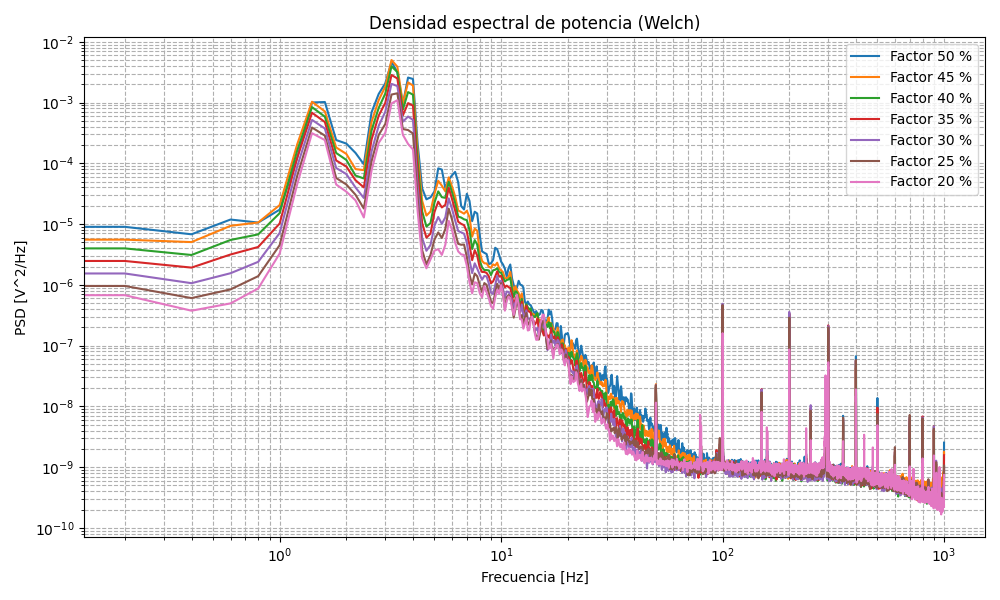
\includegraphics[width=0.97\linewidth]{Figures/25_08_2025/Espectros_variando_amplitud}
	\caption{PSDs para las distintas amplitudes de forzado en la banda de 0 a 4 Hz en la cuba chica.}
	\label{fig:espectrosvariandoamplitud}
\end{figure}


Además se pueden calcular los exponentes en cada rango al hacer un ajuste lineal (usé de 4 a 13 Hz para gravedad y de 20 a 35 Hz para capilar) y comparar con los teóricos (-4 para gravedad y -17/6 para capilar). Notamos que como le pasa a \cite{falconObservationGravityCapillaryWave2007} hay una dependencia importante con la amplitud del forzado de ambos exponentes. 

Por último después de los ajustes lineales se puede sacar la frecuencia de cruce entre regímenes, que teóricamente sale de pedir: 

\begin{equation}
	gk \sim \frac{\gamma}{\rho}k^3 
\end{equation}

Esto da aproximadamente 13.4 Hz. Y vemos que en general sí tiende a eso. 

\begin{figure}[th!]
	\centering
	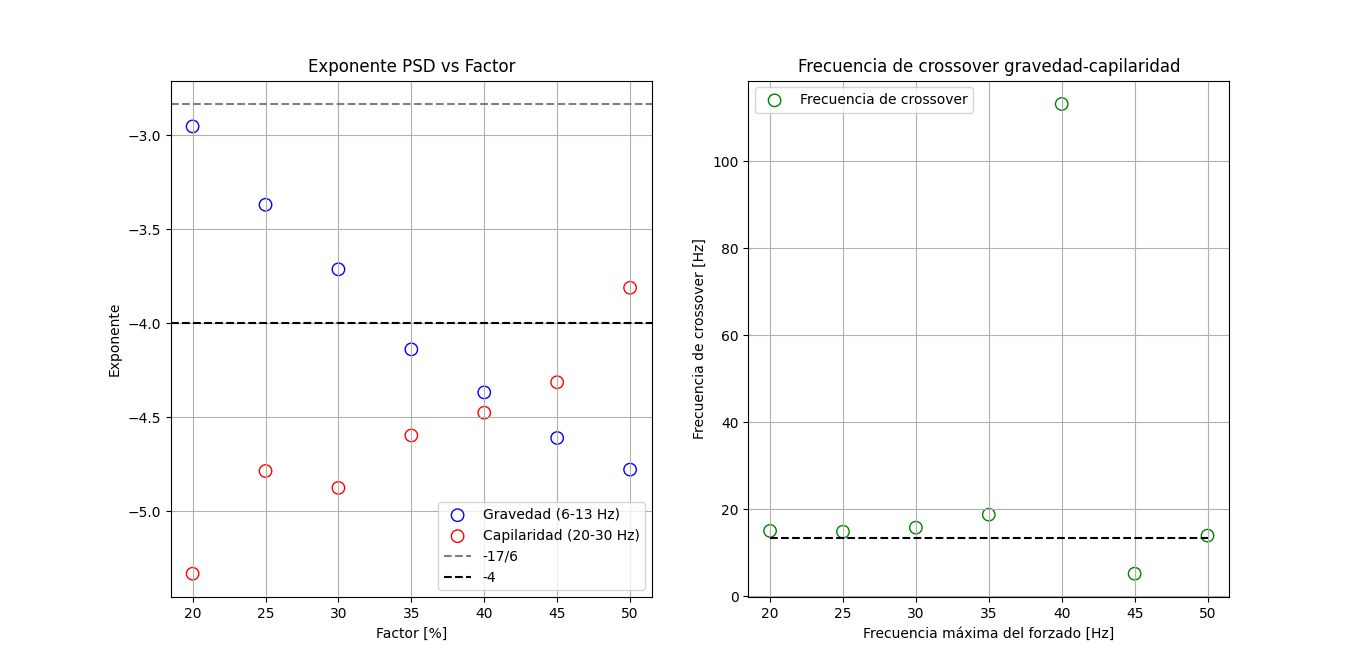
\includegraphics[width=0.769\linewidth]{Figures/25_08_2025/Espectros_variando_amplitud_exponentes}
	\caption{Exponentes de las distintas regiones de las PSDs y frecuencias de cruce al variar la amplitud del forzado.}
	\label{fig:espectrosvariandoamplitudexponentes}
\end{figure}

Más abajo lo mismo que antes pero para amplitud constante y variando la banda de frecuencias. 

\begin{figure}[th!]
	\centering
	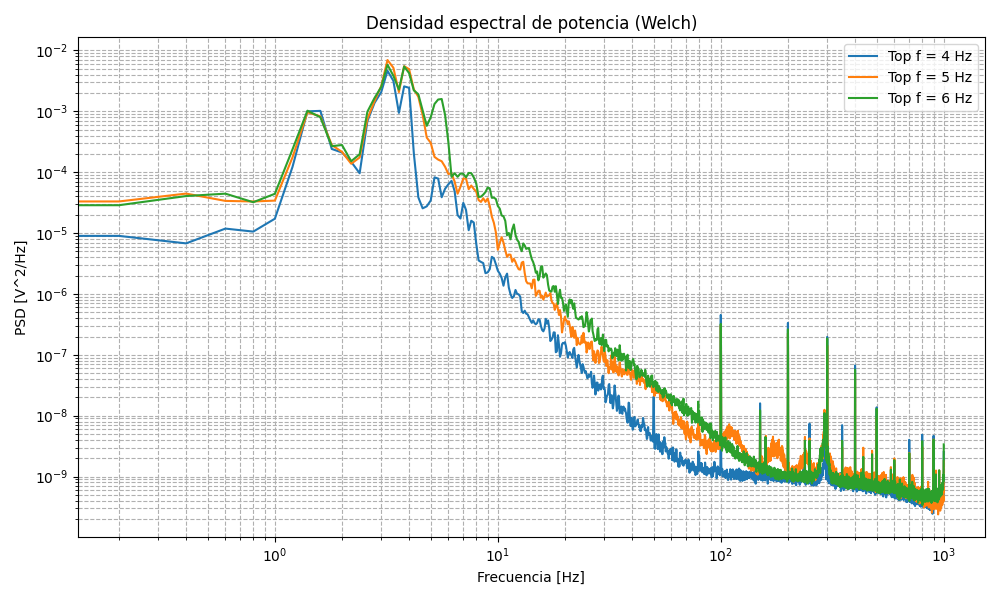
\includegraphics[width=0.97\linewidth]{Figures/25_08_2025/Espectros_variando_frecuencia}
	\caption{PSDs para las distintas bandas de frecuencia de forzado para amplitud constante de 50 \% en la cuba chica.}
	\label{fig:espectrosvariandofrecuencia}
\end{figure}

Notamos que la frecuencia de cruce acá empieza a aumentar bastante. 


\begin{figure}[th!]
	\centering
	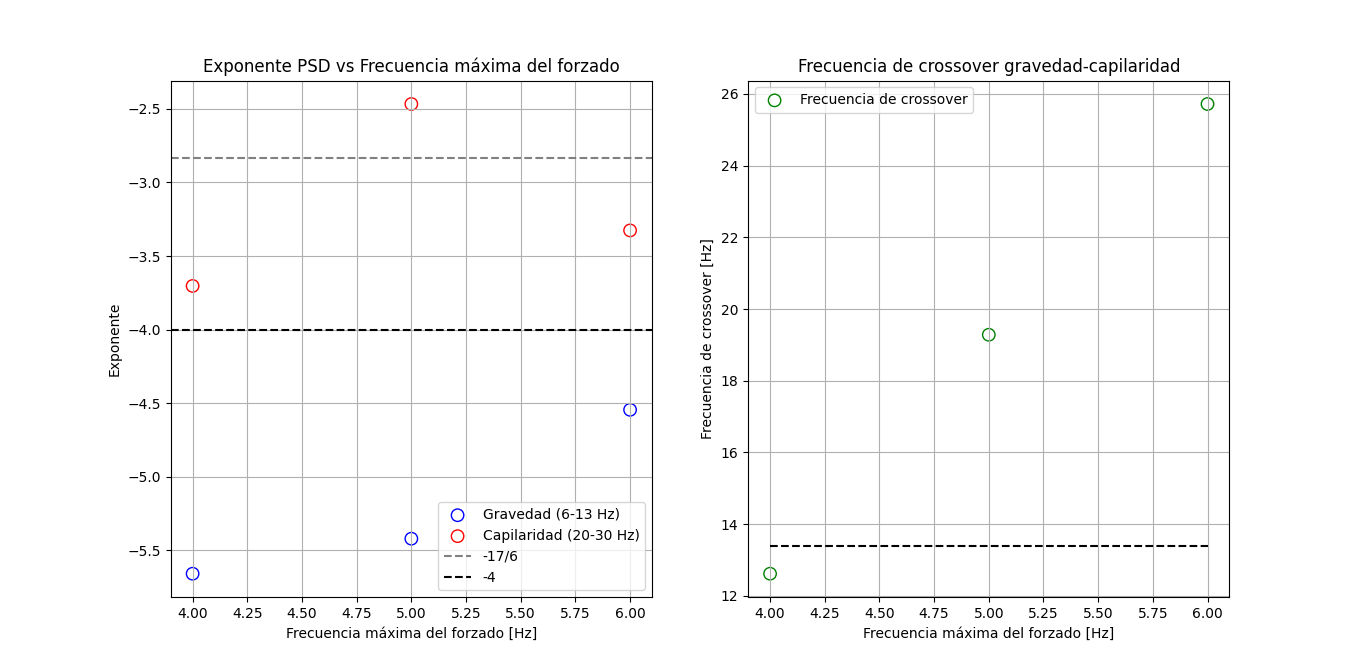
\includegraphics[width=0.769\linewidth]{Figures/25_08_2025/Espectros_variando_frecuencia_exponentes}
	\caption{Exponentes de las distintas regiones de las PSDs y frecuencias de cruce al variar la banda de frecuencia.} 
	\label{fig:espectrosvariandofrecuenciaexponentes}
\end{figure}


\section{Intermitencia.} % * 

Acá seguí los procedimientos detallados en \cite{falconObservationIntermittencyWave2007}. Cuando hable de \textit{primeras diferencias} estoy haciendo: 

\begin{equation}
	\Delta\eta(\tau) = \eta(t + \tau) - \eta(t) 
\end{equation} 

Y cuando hable de \textit{segundas diferencias} que es en lo que se enfocan principalmente estoy haciendo: 

\begin{equation}
	\Delta\eta(\tau) = \eta(t + \tau) - 2\eta(t) + \eta(t - \tau) 
\end{equation}

Y en todos los casos por función de estructura de orden $p$ estoy usando su definición: 

\begin{equation}
	S_p(\tau) = \langle |\Delta\eta|^p \rangle_t
\end{equation}

\subsubsection*{PDFs de las $\Delta\eta$.} 
Para estas realicé las PDFs por ventanas de la serie temporal (de 60 segundos con un 75 \% de overlap) y después las promedié todas. En todos casos está normalizado por la desviación estándar y tienen media 0. 

\begin{figure}[!ht]
	\begin{minipage}[c]{0.32335\textwidth}
			\begin{subfigure}{\textwidth}
					\centering
					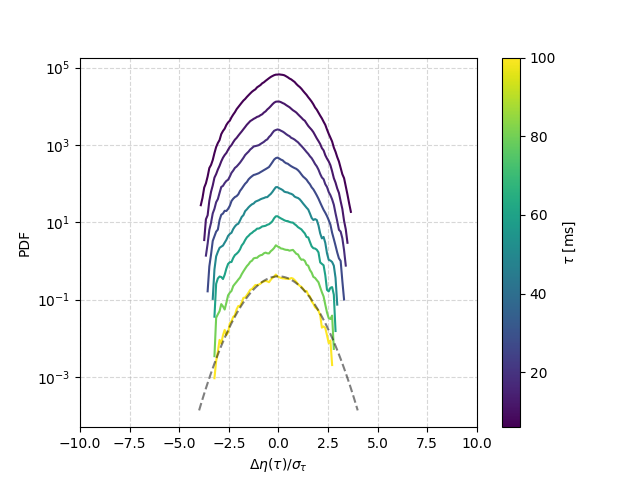
\includegraphics[width=0.98\textwidth]{Figures/25_08_2025/Primeras_diferencias_0_4Hz_amp20.png}
					\captionsetup{width=0.958\textwidth}
					\subcaption{Banda 0-4 Hz, amplitud 20 \%.}
				\end{subfigure}
		\end{minipage}\begin{minipage}[c]{0.323349\textwidth}
			\begin{subfigure}{\textwidth}
					\centering
					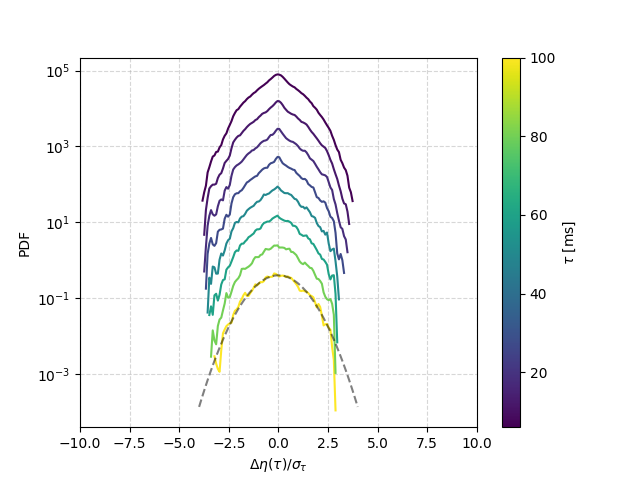
\includegraphics[width=0.98\textwidth]{Figures/25_08_2025/Primeras_diferencias_0_4Hz_amp50.png}
					\captionsetup{width=0.958\textwidth}
					\subcaption{Banda 0-4 Hz, amplitud 50 \%.}
				\end{subfigure}
		\end{minipage}\begin{minipage}[c]{0.323349\textwidth}
			\begin{subfigure}{\textwidth}
				\centering
				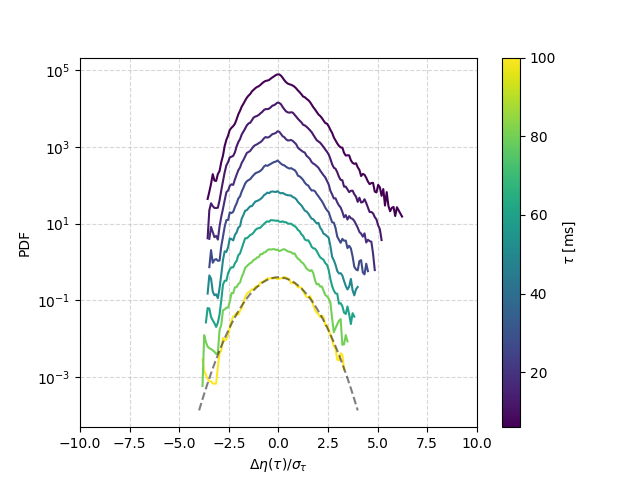
\includegraphics[width=0.98\textwidth]{Figures/25_08_2025/Primeras_diferencias_0_6Hz_amp50.png}
				\captionsetup{width=0.958\textwidth}
				\subcaption{Banda 0-6 Hz, amplitud 50 \%.}
			\end{subfigure}
		\end{minipage}
	\caption{Primeras diferencias para distintas mediciones y tiempos de delay $\tau$.}
	\label{fig:primeras_diferencias_pdfs}
\end{figure}   

\begin{figure}[!ht]
	\begin{minipage}[c]{0.32335\textwidth}
		\begin{subfigure}{\textwidth}
			\centering
			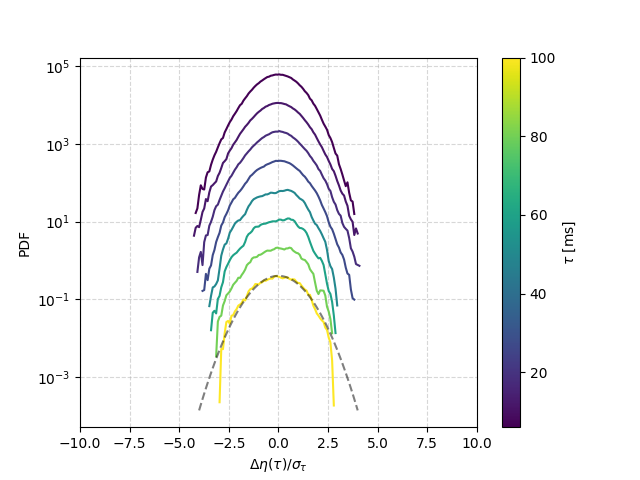
\includegraphics[width=0.98\textwidth]{Figures/25_08_2025/Segundas_diferencias_0_4Hz_amp20.png}
			\captionsetup{width=0.958\textwidth}
			\subcaption{Banda 0-4 Hz, amplitud 20 \%.}
		\end{subfigure}
	\end{minipage}\begin{minipage}[c]{0.323349\textwidth}
		\begin{subfigure}{\textwidth}
			\centering
			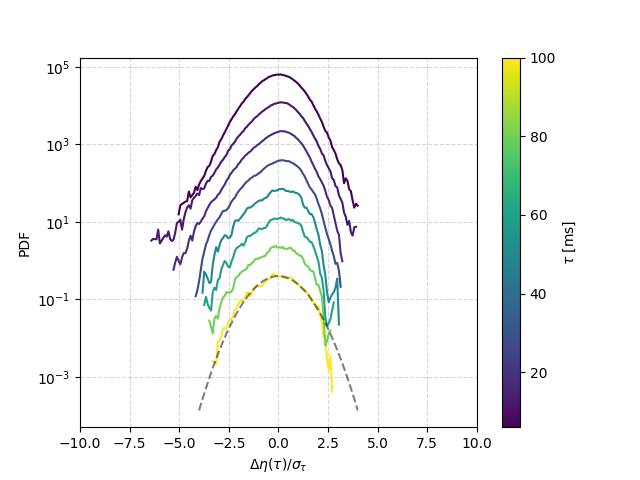
\includegraphics[width=0.98\textwidth]{Figures/25_08_2025/Segundas_diferencias_0_4Hz_amp50.png}
			\captionsetup{width=0.958\textwidth}
			\subcaption{Banda 0-4 Hz, amplitud 50 \%.}
		\end{subfigure}
	\end{minipage}\begin{minipage}[c]{0.323349\textwidth}
		\begin{subfigure}{\textwidth}
			\centering
			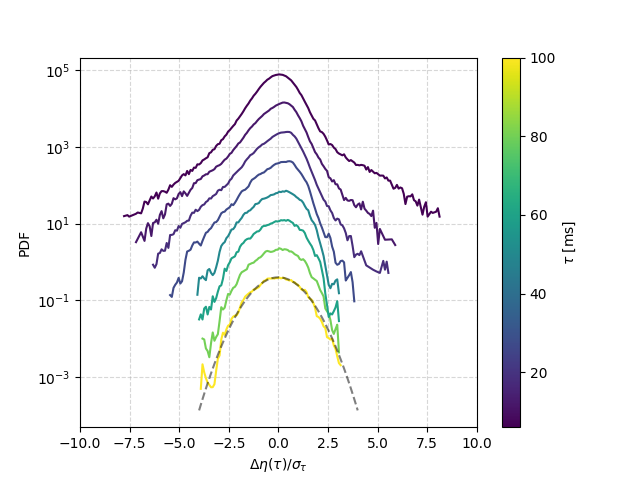
\includegraphics[width=0.98\textwidth]{Figures/25_08_2025/Segundas_diferencias_0_6Hz_amp50.png}
			\captionsetup{width=0.958\textwidth}
			\subcaption{Banda 0-6 Hz, amplitud 50 \%.}
		\end{subfigure}
	\end{minipage}
	\caption{Segundas diferencias para distintas mediciones y tiempos de delay $\tau$.}
	\label{fig:segundas_diferencias_pdfs}
\end{figure} 


\subsubsection*{Tiempo de correlación y funciones de estructura.}
Acá para hacer el promedio temporal no usé ventanas como antes sino que usé la serie temporal completa directamente, de unos 4 minutos sampleada a 2 kHz.

\begin{figure}[th!]
	\centering
	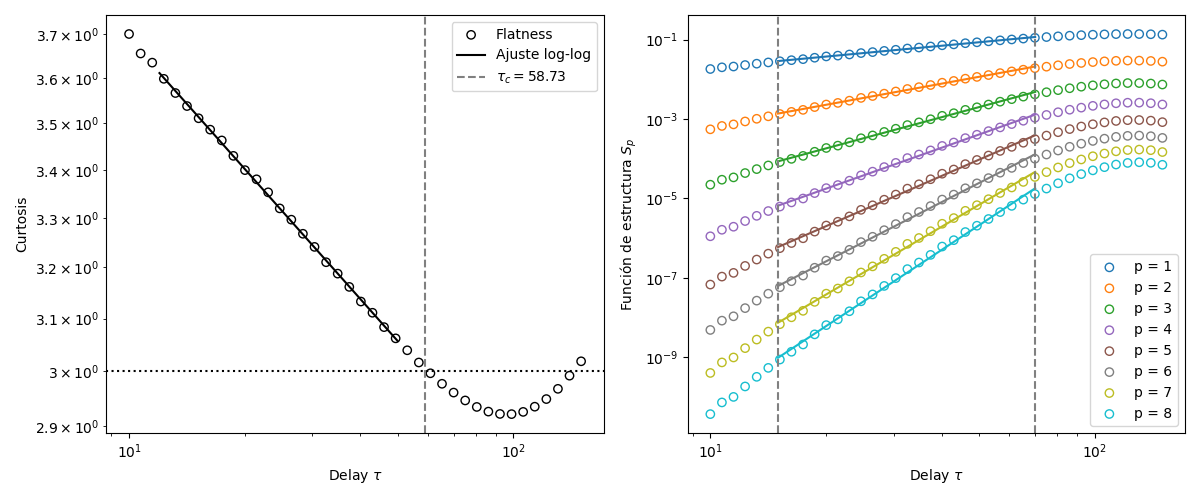
\includegraphics[width=0.87\linewidth]{Figures/25_08_2025/Primeras_diferencias_Funciones_de_estructura_0_6Hz_50}
	\caption{Flatness y funciones de estructura para las primeras diferencias ajustadas linealmente en log-log. La pendiente de $S_4/S_2^2$ es $\alpha$ = -0.117 y el tiempo de correlación $\tau_c$ = 58.726 ms.}
	\label{fig:primerasdiferenciasfuncionesdeestructura06hz50}
\end{figure} 


\begin{figure}[th!]
	\centering
	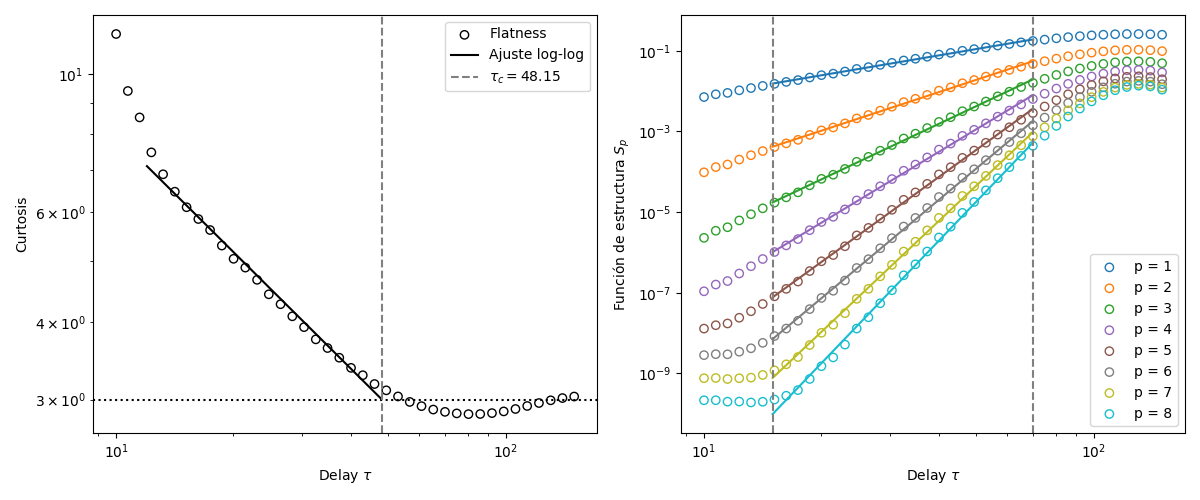
\includegraphics[width=0.87\linewidth]{Figures/25_08_2025/Segundas_diferencias_Funciones_de_estructura_0_6Hz_50}
	\caption{Flatness y funciones de estructura para las segundas diferencias ajustadas linealmente en log-log. La pendiente de $S_4/S_2^2$ es $\alpha$ = -0.621 y el tiempo de correlación $\tau_c$ = 48.146 ms.}
	\label{fig:segundasdiferenciasfuncionesdeestructura06hz50}
\end{figure}

Por análisis dimensional muestran en \cite{falconObservationIntermittencyWave2007} que la pendiente del \textit{flatness} debería ser $\alpha$ = 4 $c_2$ que si bien no se cumple exactamente da bastante cerca. 

\subsubsection*{Exponentes de las funciones de estructura.}
\begin{figure}[!ht]
	\begin{minipage}[c]{0.5\textwidth}
		\begin{subfigure}{\textwidth}
			\centering
			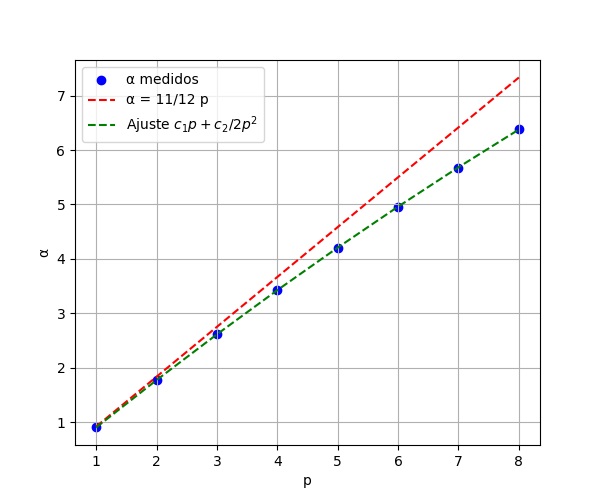
\includegraphics[width=0.88\textwidth]{Figures/25_08_2025/Primeras_diferencias_potencias_0_6Hz_50.png}
			\captionsetup{width=0.98\textwidth}
			\subcaption{Primeras diferencias ($c_1$ = 0.915 y $c_2$ = 0.029).}
		\end{subfigure}
	\end{minipage}\begin{minipage}[c]{0.49\textwidth}
		\begin{subfigure}{\textwidth}
			\centering
			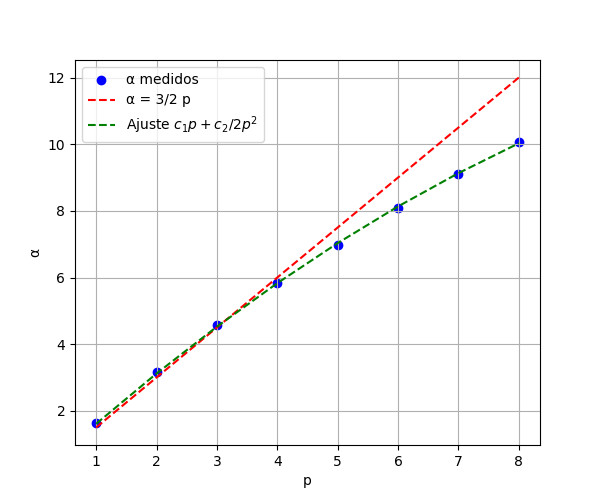
\includegraphics[width=0.98\textwidth]{Figures/25_08_2025/Segundas_diferencias_potencias_0_6Hz_50.png}
			\captionsetup{width=0.958\textwidth}
			\subcaption{Segundas diferencias ($c_1$ = 1.661 y $c_2$ = 0.102).}
		\end{subfigure}
	\end{minipage}
	\caption{Pendientes de la ley de potencias para las funciones de estructura en función del orden $p$ para las primeras y segundas diferencias. En rojo la predicción teórica por análisis dimensional y en verde un ajuste cuadrático de la forma $f(p) = c_1 p - \frac{c_2}{2}p^2$}
	\label{fig:potenicas_segun_funcion_de_Estructura}
\end{figure} 




%\begin{figure}[!ht]
%	\begin{minipage}[c]{0.5\textwidth}
	%		\begin{subfigure}{\textwidth}
		%			\centering
		%			\includegraphics[width=0.8\textwidth]{}
		%			\captionsetup{width=0.8\textwidth}
		%			\subcaption{.}
		%		\end{subfigure}
	%	\end{minipage}\begin{minipage}[c]{0.49\textwidth}
	%		\begin{subfigure}{\textwidth}
		%			\centering
		%			\includegraphics[width=0.8\textwidth]{}
		%			\captionsetup{width=0.8\textwidth}
		%			\subcaption{.}
		%		\end{subfigure}
	%	\end{minipage}
%	\caption{}
%	\label{fig:}
%\end{figure} 


